% Owner: Hassan Ashraf 24L-3073
\section{Evaluation}
\label{sec:evaluation}

\subsection{Validation Strategy}

All models use the chronological split from Deliverable~1
(Table~\ref{tab:splits}): training 2010--2021 (2,988 days, 71\%), validation
2022--2023 (502 days, 12\%) and test 2024--2026 (700 days, 17\%). The data is
never shuffled. A random train/test split or ordinary $k$-fold
cross-validation would let a model learn from days that come \emph{after} the
days it is tested on. Because neighbouring days share most of their 5-day
outcome window and markets move in long regimes, this leaks the future and
overstates accuracy~\cite{a_bergmeir2012}.

Inside the training split, hyperparameters are tuned with \textbf{walk-forward
cross-validation}: \texttt{TimeSeriesSplit} with five folds, where each fold
trains on all earlier data and validates on the next block. A \textbf{gap of
five days} separates each training block from its validation block, and the
last five rows of the training and validation splits are \textbf{purged} before
fitting, because their labels look into the following period. This follows the
purging practice recommended for financial data~\cite{a_lopezdeprado2018}.

The validation split is used only for model selection: choosing the feature set
of each classical model (Section~\ref{sec:classical}) and early stopping of the
LSTM (Section~\ref{sec:deep}). The test split is used once, for the final
results below.

\subsection{Metric Selection}

\textbf{Accuracy alone is misleading here.} Gold rose in 60.9\% of the 5-day
windows of the test period, so a model that always says ``up'' is right 60.9\%
of the time without learning anything. We therefore report four further metrics,
treating ``up'' as the positive class (TP, FP and FN are true positives, false
positives and false negatives):

\begin{itemize}
  \item \textbf{Precision} $= \frac{TP}{TP + FP}$: when the model says prices
        will rise, how often it is right. For a buyer this is the reliability
        of a ``buy now'' signal; low precision means buying ahead of falls.
  \item \textbf{Recall} $= \frac{TP}{TP + FN}$: the share of rising weeks the
        model catches. Low recall means many missed chances to buy before a rise.
  \item \textbf{F1} $= 2 \cdot \frac{\text{Precision} \cdot \text{Recall}}{\text{Precision} + \text{Recall}}$:
        the harmonic mean, high only when both are high.
  \item \textbf{AUC-ROC}~\cite{a_fawcett2006}: the probability that the model
        gives a randomly chosen rising week a higher score than a randomly
        chosen falling week. It does not depend on the 0.5 threshold or on the
        share of rising weeks, so it stays comparable when the class balance
        shifts between periods, as it does here (54\% up in training, 61\% in
        test). It is our main metric for model selection.
\end{itemize}

\subsection{Results}

Table~\ref{tab:test-results} compares all models on the test set (threshold
0.5). The full table for every split is in
\texttt{results/tables/model\_comparison.csv}.

\begin{table}[H]
  \centering
  \begin{tabular}{lccccc}
    \toprule
    Model & Accuracy & Precision & Recall & F1 & AUC-ROC \\
    \midrule
    Majority baseline        & 0.609 & 0.609 & 1.000 & 0.757 & 0.500 \\
    Logistic regression      & 0.498 & \textbf{0.696} & 0.311 & 0.430 & 0.569 \\
    Random forest            & 0.391 & 0.000 & 0.000 & 0.000 & 0.551 \\
    Hist.\ gradient boosting & 0.391 & 0.000 & 0.000 & 0.000 & \textbf{0.599} \\
    LSTM                     & 0.522 & 0.643 & 0.485 & 0.553 & 0.538 \\
    \bottomrule
  \end{tabular}
  \caption{Test-set results (2024--2026, 701 days, 60.9\% up).}
  \label{tab:test-results}
\end{table}

\begin{figure}[H]
  \centering
  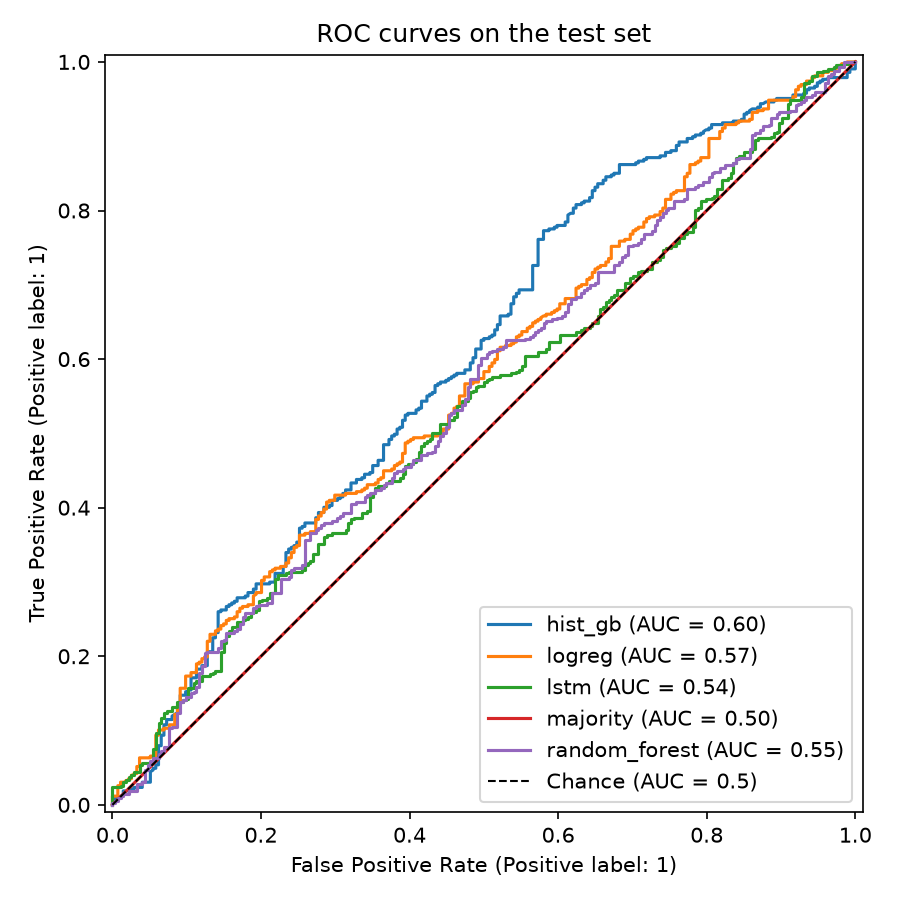
\includegraphics[width=0.55\textwidth]{evaluation/roc_test.png}
  \caption{ROC curves on the test set. The dashed line is a random guess.}
  \label{fig:roc-test}
\end{figure}

\begin{figure}[H]
  \centering
  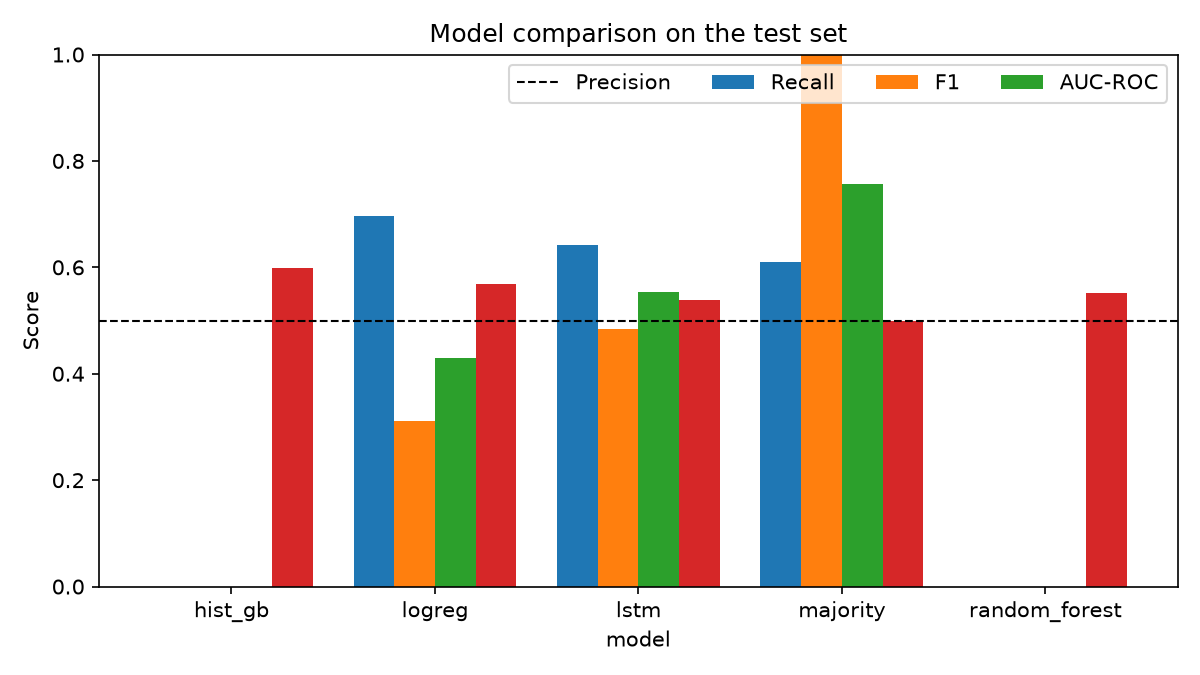
\includegraphics[width=0.85\textwidth]{evaluation/metrics_test.png}
  \caption{Precision, recall, F1 and AUC-ROC on the test set.}
  \label{fig:metrics-test}
\end{figure}

\begin{figure}[H]
  \centering
  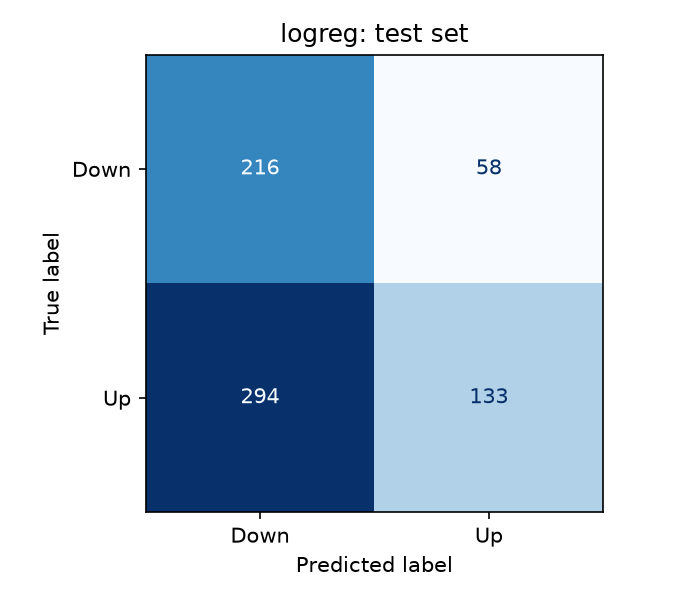
\includegraphics[width=0.32\textwidth]{evaluation/confusion_logreg.png}
  \hfill
  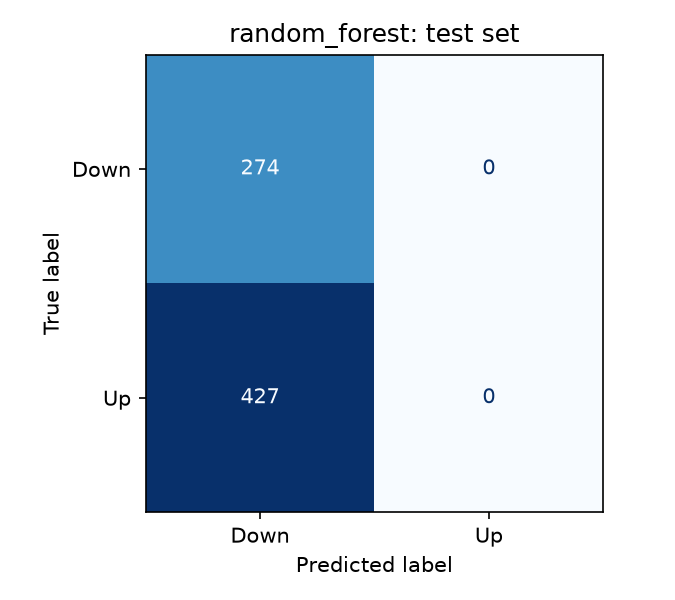
\includegraphics[width=0.32\textwidth]{evaluation/confusion_random_forest.png}
  \hfill
  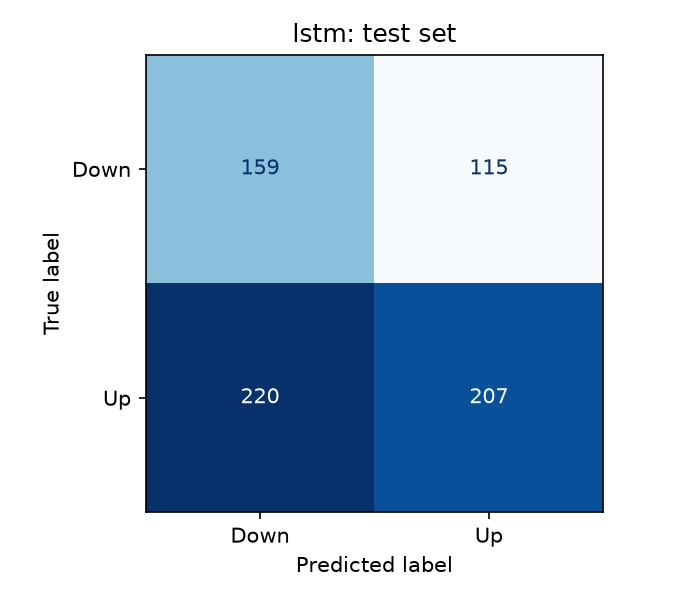
\includegraphics[width=0.32\textwidth]{evaluation/confusion_lstm.png}
  \caption{Test-set confusion matrices of logistic regression (left), random forest (middle) and the LSTM (right).}
  \label{fig:confusion}
\end{figure}

\subsection{Discussion}

\begin{itemize}
  \item \textbf{The baseline has the best accuracy and F1}, purely because most
        test weeks went up. Its AUC of 0.500 shows that it has no ability to
        tell rising from falling weeks. This is exactly why accuracy and the
        F1 of the positive class cannot be used on their own.
  \item \textbf{Logistic regression gives the most useful signal.} When it
        predicts ``up'' it is right 69.6\% of the time (133 of 191 calls),
        clearly above the 60.9\% base rate, but it is cautious and catches only
        31\% of rising weeks. For a buyer, a rare but reliable ``buy now''
        signal is more valuable than a frequent unreliable one.
  \item \textbf{The LSTM gives the most balanced predictions.} It has the
        best F1 of all learned models (0.553): it catches 48.5\% of rising
        weeks (207 of 427) with 64.3\% precision, and predicts ``up'' on 46\%
        of test days instead of collapsing to one class. It uses only the
        stationary features (Section~\ref{sec:deep}), so the rise in price
        levels does not push it to one side. Its ranking ability is weak,
        however: the AUC falls from 0.594 on validation, the best of all
        models, to 0.538 on test, another sign that the relationship between
        features and direction changed between periods.
  \item \textbf{The tree models predict ``down'' on every one of the 701 test
        days} (recall 0, Figure~\ref{fig:confusion}), even though their AUC
        (0.551 and 0.599) shows that they still rank the days better than
        chance. All their test probabilities lie below 0.5 (at most 0.45). The
        cause is distribution shift: both models rely on price-level features
        (Figure~\ref{fig:feature-importance}), and gold traded far above its
        training range in 2024--2026 (the scaled gold level has a test mean of
        8.35 standard deviations, Section~\ref{sec:features_eda}). Trees cannot
        extrapolate, so every test day falls into the leaves for the highest
        prices seen in training, which were mostly followed by falls.
        Section~\ref{sec:error-bias} analyses this failure in detail.
  \item \textbf{Overall, the predictable signal is small}: the best AUC is
        0.60, and no model beats the baseline's accuracy. This result is
        honest rather than disappointing: it shows that direction alone is a
        weak basis for procurement decisions, and it motivates the changes
        planned for Deliverable~3 (Section~\ref{sec:conclusion}).
\end{itemize}